%%%%%%%%%%%%%%%%%%%%%%%%%%%%%%%%%%%%%%%%%%%%%%%%%%%%%%%%%%%
% PREAMBOLO
%%%%%%%%%%%%%%%%%%%%%%%%%%%%%%%%%%%%%%%%%%%%%%%%%%%%%%%%%%%

% === Impostazione del documento ==========================
\documentclass[12pt,a4paper,twoside,english,italian,hidelinks]{book}


\usepackage{setspace}
\onehalfspace

% === Regolazione dei margini =============================
\addtolength{\oddsidemargin}{30pt}
\addtolength{\evensidemargin}{-30pt}
\usepackage{fancyhdr}
\usepackage{multirow}
\usepackage{multicol}
\usepackage[section]{placeins}

% === Impostazione dei font ===============================

\usepackage[T1]{fontenc}
\usepackage[italian]{babel}
\usepackage{ae}
\usepackage{relsize}
\usepackage{csquotes} 
\usepackage{amsmath}
\usepackage{amsfonts}
\usepackage{mathdots}
\usepackage[colorlinks=true]{hyperref}
\hypersetup{
	bookmarksnumbered=true,
	linkcolor=black,
	citecolor=black,
	pagecolor=black,
	urlcolor=black,
}
\usepackage{verbatim}
\usepackage{alltt}

% === Integrazione delle figure ===========================
\usepackage{graphicx}
\graphicspath{{./imgs/}}
\renewcommand{\figurename}{Fig.}
\usepackage{subfigure}
\usepackage[section]{placeins}
\usepackage[nottoc]{tocbibind}

% === Per gli algoritmi ===================================
\usepackage{algorithmicx}
\usepackage[ruled]{algorithm}
\usepackage{algpseudocode}
\usepackage{listings}
\usepackage{xcolor}

%New colors defined below
\definecolor{codegreen}{rgb}{0,0.6,0}
\definecolor{codegray}{rgb}{0.5,0.5,0.5}
\definecolor{codeorange}{rgb}{0.255,0.112,0.67}
\definecolor{codepurple}{rgb}{0.58,0,0.8}
\definecolor{backcolour}{rgb}{0.250,0.250,0.250}

%Code listing style named "mystyle"
\lstdefinestyle{mystyle}{
  backgroundcolor=\color{white},   commentstyle=\color{codegreen},
  keywordstyle=\color{orange},
  numberstyle=\tiny\color{codegray},
  stringstyle=\color{codepurple},
  basicstyle=\ttfamily\tiny, %or small or footnotestyle
  breakatwhitespace=false,         
  breaklines=true,                 
  captionpos=b,                    
  keepspaces=true,                 
  numbers=left,                    
  numbersep=3pt,                  
  showspaces=false,                
  showstringspaces=false,
  showtabs=false,                  
  tabsize=1
}

%"mystyle" code listing set
\lstset{style=mystyle}

% === Per le tabelle ======================================
\usepackage{tabularx}

% === Per la bibliografia multicolonna ====================
\usepackage{etoolbox}
%\usepackage[backend=biber, sorting=none]{biblatex} \addbibresource{bibliografia-tesi.bib}

%\patchcmd{\thebibliography}{\list}{\begin{multicols}{2}\smaller\list}{}{}
%\appto{\endthebibliography}{\end{multicols}}


%%%%%%%%%%%%%%%%%%%%%%%%%%%%%%%%%%%%%%%%%%%%%%%%%%%%%%%%%%%
% TESTO DELLA TESI
%%%%%%%%%%%%%%%%%%%%%%%%%%%%%%%%%%%%%%%%%%%%%%%%%%%%%%%%%%%

\begin{document}
\frontmatter
	% === Frontespizio ====================================
	\pagestyle{empty}
	%%%%%%%%%%%%%%%%%%%%%%%%%%%%%%%%%%%%%%%%%%%%%%%%%%%%%%%%%%%
% Frontespizio
%%%%%%%%%%%%%%%%%%%%%%%%%%%%%%%%%%%%%%%%%%%%%%%%%%%%%%%%%%%

\begin{titlepage}
 \begin{center}
     
\includegraphics[width=3.5cm]{imgs/unimol/unimol_color.png}\\
     \vspace{1em}
     {\Large \textsc{Università  degli studi del Molise}}\\
     \vspace{1em}
     {\Large \textsc{Dipartimento di Bioscienze e Territorio}}\\
     \vspace{1em}
      {\Large \textsc{Corso di Laurea in Informatica}}\\
     \vspace{2em}
     {\normalsize Tesi di Laurea in}\\
     \vspace{1em}
     {\Large \textsc{Programmazione Web e Mobile}}\\
     \vspace{3em}
     {\LARGE\textbf{
     TITOLO TITOLO TITOLO\\\vspace{0.4em}
     	TITOLO TITOLO TITOLO
     }}\\
 \end{center}

%spazio tra il titolo e i nomi%
\vskip 1.2cm
  \begin{center}
    \begin{tabular}{c c c c c c c c}
      Relatore & & & & & & & Candidato \\[0.2cm]
      \large{Ing. Francesco Mercaldo} & & & & & & & \large{Andrea D'Aguanno} \\ & & & & & & & {Matricola: 156708}\\[0.4cm] 
       Correlatore & & & & & & & \\[0.2cm]
      \large{Dott.ssa Rosangela Casolare}& & & & & & & \\
    \end{tabular}
  \end{center}

\vskip 1.5cm
\begin{center}
{\normalsize Anno Accademico 2020/2021}
\end{center}
\end{titlepage}

\clearpage{\pagestyle{empty}\cleardoublepage}

	
	%%% inseriamo apgina vuota %%%
	%\clearpage
    %\null
    %\thispagestyle{empty}
    %\clearpage
	%%%%%%%%%%%%%%%%%%%%%%%%%%%%%%%
	%%%%%%%%%%%%%%%%%%%%%%%%%%%%%%%%%%%%%%%%%%%%%%%%%%%%%%%%%%%
% Dedica

\vspace{5em}
\begin{flushright}
  {\normalsize \textit{Ai miei genitori.}}\\
  {\normalsize \textit{Grazie.}}\\
\end{flushright}

\clearpage{\pagestyle{empty}\cleardoublepage}


	% === Indice ==========================================
	\tableofcontents
	\listoffigures
	


	% === Capitoli Tesi ===================================
	\pagestyle{plain}
	%%%%%%%%%%%%%%%%%%%%%%%%%%%%%%%%%%%%%%%%%%%%%%%%%%%%%%%%%%%
\mainmatter %inizia la numeraizione da capo
\chapter{Introduzione}
\label{chap:Introduzione}

%%%%%%%%%%%%%%%%%%%%%%%%%%%%%%%%%%%%%%%%%%%%%%%%%%%%%%%%%%%

\section{Contesto applicativo}
\label{sec:intro1}
Nell'ambito della sicurezza informatica, attraverso il termine malware, abbreviazione di \textit{malicious software}, si vanno ad indicare tutti quei "software malevoli" il cui scopo ultimo è di andare ad interferire con le operazioni svolte da un utente in un dispositivo elettronico. Un malware può agire a diversi livelli, di fatti il termine stesso racchiude diverse categorie di software malevolo: Virus, Ransomware, Trojan, Worm, sono solo alcuni dei possibili tipi di malware. La caratteristica che differenzia un malware da un qualsiasi altro applicativo software risiede nell'intenzionalità dello sviluppatore nel voler realizzare codice malevolo, quindi non rientrano in questo contesto tutti quei software che presentano un bug che mina alla sicurezza dell'applicativo. 
\\È dunque fondamentale studiare i rischi ed i pericoli che riguardano il mondo dell'informatica e più nello specifico quello del mobile computing\footnote{Con il termine mobile computing, si vanno ad indicare tutti quei dispositivi che non sono vincolati dall'utilizzo in una posizione fissa. Rientrano in questa categoria anche i dispositivi mobile come gli smartphone}. Uno dei sistemi operativi più diffusi per i dispositivi mobile è "Android" che grazie alla sua flessibilità permette all'utente di eseguire particolari azioni liberamente all'interno del proprio ecosistema. Android  ad oggi è leader del mercato degli smartphone, ed è quindi il sistema operativo più utilizzato a livello mondiale con 2,5 miliardi di utenti attivi mensilmente nella prima metà del 2019\cite{venturebeat}. La sua diffusione è stata incentivata anche perché non è collegato con un produttore hardware specifico portando il sistema operativo di Google ad avere solo nel 2015 più di quattromila dispositivi diversi che utilizzassero android\cite{4000}. 





%%%%%%%%%%%%%%%%%%%%%%%%%%%%%%%%%%%%%%%%%%%%%%%%%%%%%%%%%%%

\section{Motivazioni e obiettivi}
\label{sec:intro2}
La possibilità di flessibilità dell'ecosistema Android apre le porte ad una maggior intrusione di codice malevolo all'interno degli applicativi, si pensi che oltre alla possibilità di istallare applicazioni dallo store ufficiale \textit{Google Play} è possibile scaricare ed istallare applicazioni attraverso il reperimento di un qualsiasi file \textit{.apk}\footnote{L'estensione apk - Android Package indica un pacchetto contenete tutti i file relativi ad una applicazione Android.} da un generico sito web. Gran parte dei malware Android si diffonde proprio attraverso l'utilizzo di quest'ultima pratica di fatti, scaricando applicazioni da siti terzi non è garantita una preventiva scansione del download per rilevarne la dannosità come avviene attraverso l'utilizzo dello store ufficiale, più nello specifico attraverso l'utilizzo di \textit{Google Play Protect} attivo di default in \textit{Google Play}.
\\Da qui la motivazione che ci ha portato allo sviluppo di questa tesi è legata alla classificazione di queste minacce, partendo da file apk, con l'obiettivo di utilizzare tecniche di machine learning, nello specifico multiple instance learning per la classificazione di applicativi colludenti affetti da malware.


%%%%%%%%%%%%%%%%%%%%%%%%%%%%%%%%%%%%%%%%%%%%%%%%%%%%%%%%%%%

\section{Risultati raggiunti}
\label{sec:intro3}
Dato un file \textit{Apk} si passa alla conversione del codice binario relativo in un file audio, nello specifico un file \textit{Wav}\footnote{L'estensione wav - Waveform Audio File Format è uno standard di formato di file audio, sviluppato da IBM e Microsoft, per memorizzare un flusso di bit audio. \cite{enwiki:1020662001}}, di seguito si passa ad una suddivisione ricavando quindi da un singolo audio più file audio. Da ognuno si è passati all'estrazione di alcune delle caratteristiche che lo compongono. Creando un dataset ad hoc, abbiamo addestrato modelli di multiple instance learning per la classificazione di applicazioni sicure o applicazioni colludenti affette da malware. 


%%%%%%%%%%%%%%%%%%%%%%%%%%%%%%%%%%%%%%%%%%%%%%%%%%%%%%%%%%%

\section{Organizzazione della tesi}
\label{sec:intro4}
La tesi è sviluppata progressivamente nei seguenti capitoli, ai quali va ad aggiungersi il capitolo corrente relativo all'introduzione:


\begin{itemize}
    \item\hyperref[chap:cap2]{\textbf{Capitolo 2}} Android \textbf{TODO: INTEGRARE}
    \item\hyperref[chap:cap3]{\textbf{Capitolo 3}} Sicurezza in ambiente Android \textbf{TODO: INTEGRARE}
    \item\hyperref[chap:cap4]{\textbf{Capitolo 4}} Metodologie \textbf{TODO: INTEGRARE}
    \item\hyperref[chap:cap5]{\textbf{Capitolo 5}} Sperimentazioni\textbf{TODO: INTEGRARE}
    \item\hyperref[chap:conclusioni]{\textbf{Capitolo 5}} Conclusione\textbf{TODO: INTEGRARE}
\end{itemize}


	%%%%%%%%%%%%%%%%%%%%%%%%%%%%%%%%%%%%%%%%%%%%%%%%%%%%%%%%%%%

\chapter{Android}
\label{chap:cap2}

Nell'ultimo decennio, il numero di utenti che utilizza dispositivi mobile è progressivamente aumentato. Questo trend è dovuto ad un aumento dell'affidabilità e delle prestazioni, si hardware che software. Ad oggi gli utenti che utilizzano uno smartphone in tutto il mondo supera i tre miliardi di persone, questo numero è destinato a salire di diverse centinaia di milioni nel costo dei prossimi anni, una stima suggerisce che nel 2023 gli utenti che utilizzeranno questo strumento sarà di circa 4,3 miliardi\cite{numberofuser}, come si può osservare in figura \ref{fig:WordwideNewzoo}.
\begin{figure}[h]
\centering 
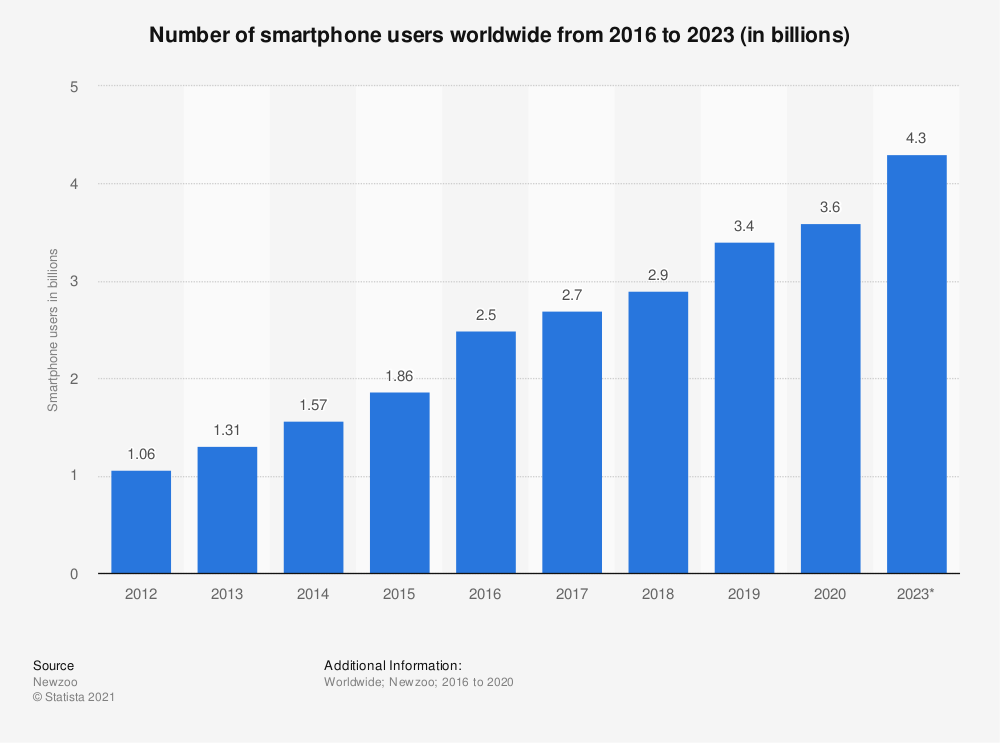
\includegraphics[width=0.7\linewidth]{imgs/capitolo2/intro/statistic_id330695_smartphone-users-worldwide-2016-2023.png} 
\caption{ Worldwide; Newzoo; 2016 to 2020} 
\label{fig:WordwideNewzoo} 
\end{figure}

Tra i sistemi operativi più utilizzati c'è il sistema operativo \textit{Android} basti pensare che nel solo anno del 2020, il 71.41\% dei dispositivi mobile, nello specifico tablet e smartphone, venduti aveva come sistema operativo proprio \textit{Andorid}, che insisme ad iOS, hanno coperto il 99.37\% del mercato mobile come si può osservare in figura \ref{fig:ww-sel}. L'ultima versione di questo sistema operativo \textit{Android R - Andorid 11} è stata rilasciata nel settembre 2020, ma la successiva versione Beta di \textit{andorid 12} è prossima al rilascio. 
\begin{figure}[h]
\centering 
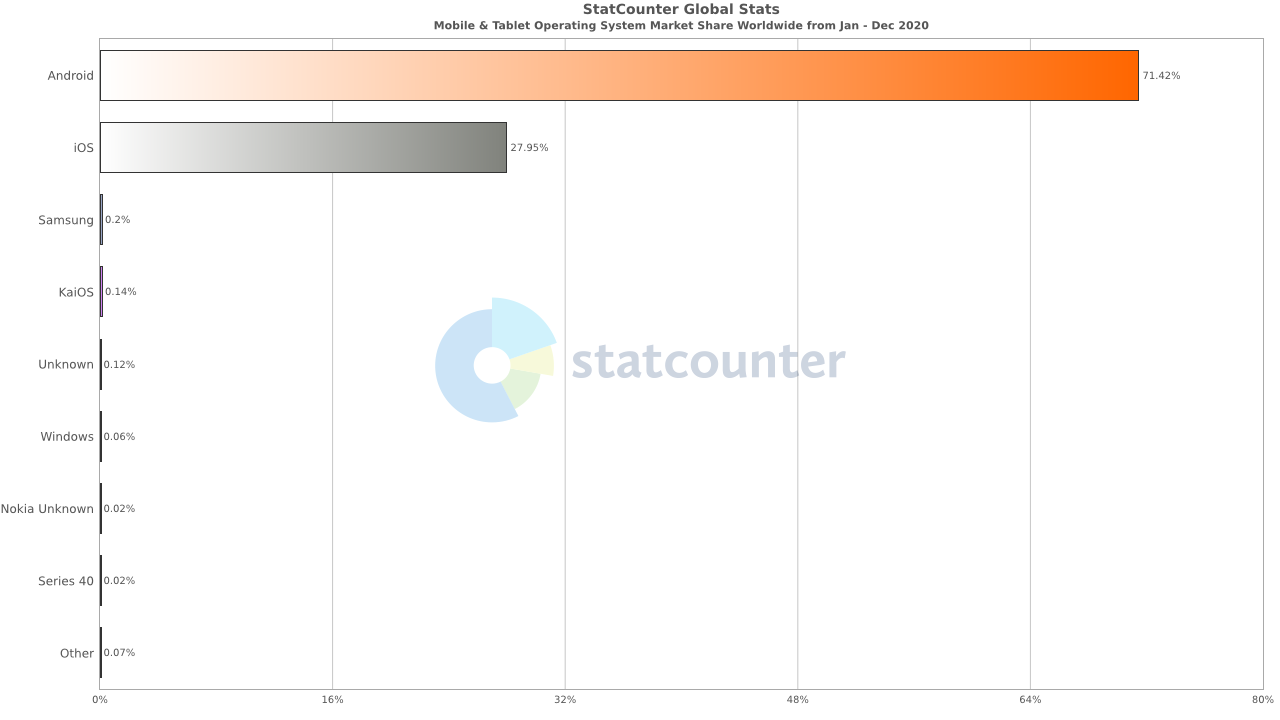
\includegraphics[width=0.7\linewidth]{imgs/capitolo2/intro/StatCounter-os_combined-ww-monthly-202001-202012-bar.png}
\caption{Mobile \& Tablet Operating System Market Share Worldwide} 
\label{fig:ww-sel} 
\end{figure}
\FloatBarrier
 La diffusione del sistema operativo \textit{Andorid} è avvenuta per mezzo di smartphone e tablet, ma sono state sviluppate soluzioni ottimizzare per dispositivi specifici come \textit{Wear Os} per smartwatch, \textit{Android TV} per smart tv, \textit{Android Auto} per l'integrazione tra smartphone ed auto, che ne aumentano ulteriormente il bacino di utenza. 
\\
Nei prossimi paragrafi esporremo l'architettura del sistema operativo \textit{Android} ed i principali componenti che formano un applicativo Android. Infine descriveremo i file apk.  

%%%%%%%%%%%%%%%%%%%%%%%%%%%%%%%%%%%%%%%%%%%%%%%%%%%%%%%%%%%

\section{Il sistema operativo}
\label{sec:Il sistema operativo}
Come già detto in precedenza Android è un sistema operativo per dispositivi mobile, sviluppato dall'azienda \textit{Android, Inc.} che fu poi acquistata nel 2005 dalla statunitense Google che lo ha poi diffuso nel 2008. Il modello di sviluppo è open source, questo consente a chiunque sia interessato di progettare e sviluppare componenti software ad esso dedicati, anche grazie alle librerie e alla documentazione fornita dal produttore. Inoltre essendo distribuito con licenza \textit{Apache 2.0} consente a chiunque di modificare e distribuire il codice sorgente. Le applicazioni sviluppate per dispositivi Android sono scritte in linguaggio Java o Kotlin, linguaggi molto diffusi che consentono di prendere parte alla progettazione di applicazioni a molti sviluppatori, questo per far si che siano sempre molte ed aggiornate le funzionalità di un dispositivo. 

\subsection{L'architettura}
L'architettura andorid può essere suddivisa in più livelli come in figura\ref{fig:andoridStack}. 
\begin{figure}[h]
\centering 
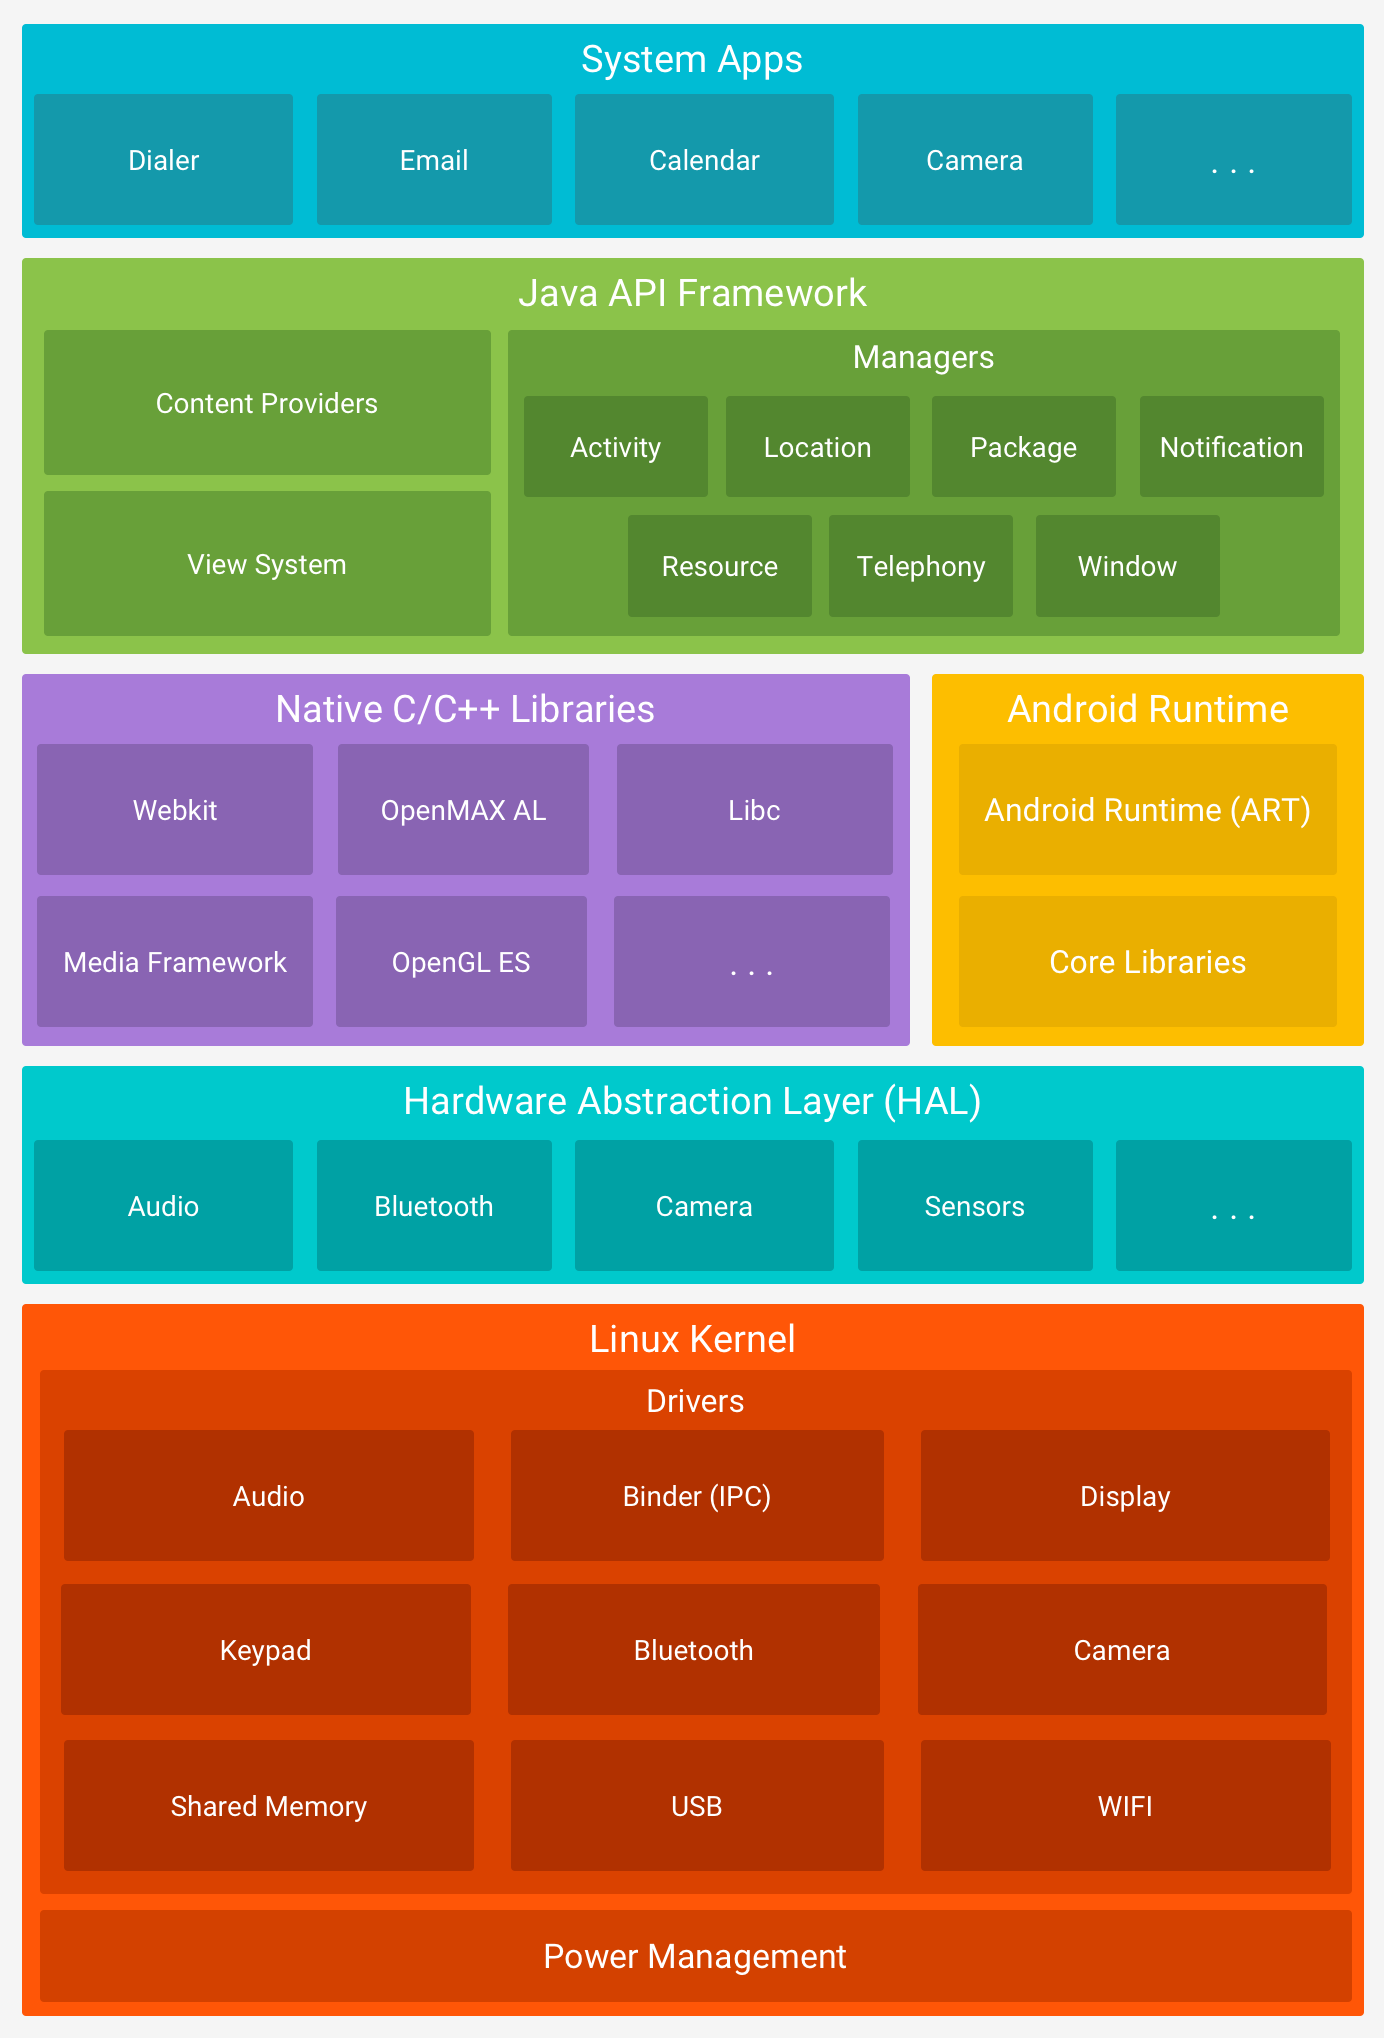
\includegraphics[width=0.4\linewidth]{imgs/capitolo2/os/android-stack_2x.png}
\caption{Android architecture} 
\label{fig:andoridStack} 
\end{figure}

\begin{itemize}
\item Nel livello più basso troviamo il \textbf{kernel linux} al quale Android si appoggia per i servizi del sistema centrale quali, sicurezza, gestione della memoria. Inoltre presenta dei driver specifici per la gestione dell'hardware. Il Kernel funge quindi da strato di comunicazione tra hardware e software.
\\Driver Binder(IPC): Questo sistema consente al sistema operativo la comunicazione tra i processi gestendo il passaggio dei dati tra le applicazioni che in Android sono eseguite ognuna in un processo differente;
\\Driver Shared Memory: consente la creazione, la mappatura ed il controllo della protezione della memoria condivisa tra i diversi processi. 

Nonostante la scelta di utilizzare un kernel linux, per ottenre affidabilita e garantire sicurezza, Andoroid è considerato come una distribuzione embedded Linux, sviluppata appositamente per ottimizzare al meglio le risorse, spesso esigue, di un dispositivo mobile e non è quindi una distribuzione Unix-like, ovvero non fa parte di tutti quei sistemi operativi simili discendenti dal sistema operativo Unix. 
\item Salendo di livello troviamo una serie di \textbf{libreirie native} sviluppate in C / C++ e libreire sviluppate in Java: 
\\\textbf{Media Framework}: è la componente in grado di gestire diversi CODEC per i vari formati di acquisizione e riproduzione di audio e video. È basata sulla libreira open surce OpenCORE. Supporta anche formati immagini come png e jpg. 
\\\textbf{Surface Manager}: Gestisce l’accesso alle funzionalità del display e coordina le diverse finestre che le applicazioni vogliono visualizzare sullo schermo, permettendo la visualizzazione contemporanea di grafica 2D e 3D dalle diverse applicazioni.
\\\textbf{OpenGL ES}: Attraverso le API implementate in questa libreria si possono gestire le funzionalità 2D e 3D e l'utilizzo di un eventuale acceleratore grafico. 
\\\textbf{SQLite}: Libreria che implementa un database relazionale.
\\\textbf{WebKit}: Browser utilizzato da Android per la visualizzazione di risosrse web. 
\\\textbf{Libc (System C library)}: Implementazione della libreria standard C system (libc), per i dispositivi basati su Linux embedded ad eempio Android.
\\\textbf{Secure Socket Layer (SSL)}: Si occupa della sicurezza attraverso la gestione dei Secure Socket Layer. Sono protocolli crittografici che permettono una comunicazione sicura e una integrità dei dati su reti TCP/IP. I SSL cifrano la comunicazione dalla sorgente alla destinazione a livello di trasporto.
\item \textbf{L'Android runtime (ART)} è un runtime system software che ha sostituito la Dalvik virtual machine (DVM), quest'ultima infatti si occupava di compilare il codice ad ogni esecuzione di un'applicazione incidendo sulle prestazioni del dispositivo. Con ART invece la compilazione del codice avviene durante l'istallazione dell'applicazione, questo comporta tempi più lunghi per la procedura di istallazione ma una volta terminata, l'esecuzione dell'applicativo non necessita di compilazione. Per mantenere la compatibilità con le versioni precedenti, il bytecode utilizzato da ART per la compilazione è lo stesso utilizzato da DVM ovvero quello fornito dal file \textit{.dex}\footnote{Le applicazioni Android sono comunemente scritti in Java e successivamente compilati in bytecode per la macchina virtuale Java, che viene quindi tradotto in bytecode Dalvik e archiviato in file .dex (Dalvik EXecutable ) oppure .odex (Optimized Dalvik EXecutable)}
\item \textbf{Java API Framework} Consiste di Api e componenti sviluppate in Java per l'esecuzione di precise funzionalità di un'applicazione Android. 
\\\textbf{Activity Manager} Responsabile dell'organizzazione della schermate in uno stack. Rappresenta lo strumento attraverso il quale avviene l'interazione con l'utente. 
\\Attraverso il \textbf{{Content Provvider}} si vanno a gestire gli accessi ai dati archiviati dalla stessa applicazione o da terze, fornisce quindi meccanismi per la condivisione di dati tra applicazioni. 
\\\textbf{Notification Manager} implementa i metodi per inviare una notifica al dispositivo ed avvisare l'utente che qualcosa è successo in background. 
\\Con l'utilizzo del \textbf{View System} si può renderizzare la GUI (graphical user interface) attraverso l'utilizzo di pulsanti, tabelle, aree di testo e così via in modo da poter gestire gli eventi associati ad ogni elemento. Il codice è contenuto in un file di marckup .xml\footnote{XML - eXtensible Markup Language, è un metalinguaggio per la definizione di linguaggi di markup dove oltre all'utilizzo di tag prestabiliti è possibile definirne dei propri a seconda del contesto applicativo.}.
\item Il primo livello, \textbf{System Apps}, contiene tutte le applicazioni native e istallate all'interno del dispositivo Android. 
\end{itemize}


%%%%%%%%%%%%%%%%%%%%%%%%%%%%%%%%%%%%%%%%%%%%%%%%%%%%%%%%%%%

\section{Le applicazioni Android}
\label{sub:aplicationAndroid}
In questo paragrafo analizzeremo la struttura di una applicazione Andorid ed i componenti da cui è composta.
\\Lo sviluppo delle applicazioni Android può avvenire attraverso l'Ide\footnote{IDE - integrated development environment è un ambiente di sviluppo, un software che, in fase di programmazione, supporta i programmatori nello sviluppo e debugging del codice sorgente di un programma \cite{itwiki:118335792} } \href{https://developer.android.com/studio/index.html}{\textit{Android Studio}} basato su JetBrains IDEA e rappresenta l'ide principale per lo sviluppo Android di Google. I linguaggi di programmazioni utilizzati per sviluppare un applicativo Andori dcome detto anche in precedenza sono \href{https://www.java.com/it/}{Java} e \href{https://kotlinlang.org/}{Kotlin}, quest'ultimo inoltre sta diventando sempre più consigliato e diffuso in ambito Android. Lo sviluppo avviene utilizzando il kit di supporto software Android (SDK) che comprende documentazione dei metodi, un debugger, librerie software ed un emulatore, in Android studio è possibile gestire ed utilizzate queste componenti da "SDK Manager". L'attività di \textit{run} del codice può avvenire sia su un dispositivo fisico collegato tramite usb e dopo aver attivato la modalità "Debug Usb" oppure scaricando ed istallando un immagine di Android nel "AVD Manager - Android virtual devices" 

\subsection{Struttura}
La struttura che compone un progetto Android può essere suddivisa in tre moduli. Tutto il progetto sarà contenuto in una cartella \textit{app}. Al interno troveremo ulteriori directory che conterranno il codice e le risorse dell'applicativo: 
\begin{itemize}
    \item \textbf{manifest}: Le applicazioni Andorid dispongono di un file AndroidManifest.xml, in questo file vanno definite tutti i componenti sviluppati, la versione minima di API necessarie per eseguire l'applicazione, i permessi di cui necessita l'applicazione ed infine elenca le librerie esterne utilizzate nel codice.  
    \item \textbf{java}: All'interno della directory java è contenuto il codice sorgente delle componenti e della logica che va a sviluppare l'applicativo, inoltre presenta anche dei file si test
    \item \textbf{res}: Le risorse che non sono codice, come imamgini, layout xml, stringhe della GUI sono contenute all'interno di subdirectory di res, nello specifico troviamo la directory \textit{drawble} ceh conterrà le immagini, la directory \textit{layout} al suo definisce tutti i file di layout.xml associati ad ogni songolo activity e/o fragment creato. Infine in \textit{values} sono contenuti vari marcatori xml utili per la definizioni di stringhe, dimensioni, colori e stili.   
\end{itemize}
Il secondo modulo, la sezione \textit{Grandle Scripts}, comprende tutti i file utilizzati per la build del progetto
\subsection{Componenti}
Le componenti principali che compongono per l'appunto un applicativo sono quatto: Activity, Service, Content Provvider, Broadcast Reciver e Intent. 

   

    \subsubsection{Activity} Un \textbf{Activity} rappresenta l'Interfaccia utente, ogni schermata è un activity, all'interno della quale possono alternarsi dei \textit{fragment}. All'interno del codice vie effettuato l'override del metoso "onCreate" in cui viene specificato il suo layout attraverso setContentView(R.layout.activity). Le acticity in Andorid seguono un ciclo di vita ben definito come si può osservare nella figura \ref{fig:lifecicle} tratta dalla \href{https://developer.android.com/guide/components/activities/activity-lifecycle}{documentazione ufficiale.}
        \begin{figure}[h]
        \centering
        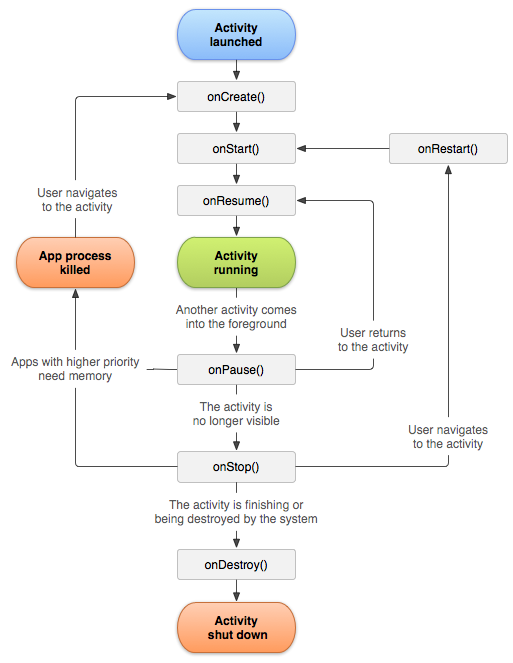
\includegraphics[width=0.35\textwidth]{imgs/capitolo2/Applicazioni/activity_lifecycle.png}
        \caption{Android lifecicle}
        \label{fig:lifecicle}
        \end{figure}
        \FloatBarrier %  evitare che i float appaiano oltre un certo punto nel tuo documento %
    Nello specifico il metodo \textit{onCreate()} viene invocato per stanziare e definire l'activity, questo viene avviato una sola volta per ciclo di vita. Successivamente quando l'activity è stata creata si invoca il metodo \textit{onStart()} che rende l'activity visibile all'utente, in modo che passi in primo piano e diventi interattiva, invocando il metodo \textit{onResume()} l'activity si pone in "ascolto" di un evento da parte dell'utente, qui definiamo l'interattività con l'user. Rimarrà in questo stato finché non accade un evento che richiede un cambio di activity (ricezione chiamata, navigazione tra activity...), il metodo invocato a questo punto sarà \textit{onPause()} che salva lo stato corrente dell'activity e dunque non sarà più possibile interagire con essa, il passo successivo comprende l'invocazione di \textit{onStop()} metodo che non rende più visibile l'activity. A questo punto l'utente può tornare all'activity ed il sistema richiamerà onResume() oppure si invocherà \textit{onDestroy()} che provvede alla pulizia e cessazione di un'activity. 

    \subsubsection{Service} Un importante componente sono i \textbf{Service}. Questi svolge operazioni in background quindi anche al di fuori dell'utilizzo diretto dell'utente dell'applicazione, difatti non ha un'interfaccia grafica. È inoltre possibile eseguire comunicazione tra processi tramite IPC. I service vanno anchessi definiti nel file AndoridManifest.xml.

    \subsubsection{Conten Provvider} Come detto in precedenza un altro componente principale è il \textbf{Content Provider} che si occupa della gestione della condivisione in memoria dei dati salvati in database , su file oppure in rete tra le applicazioni. Risulta fondamentale per il controllo delle autorizzazioni per l'accesso ai dati.
    
    \subsubsection{Broadcast reciver} Il \textbf{Broadcast reciver} è un componente che dato un messaggio a livello di sistema, in broadcast, consente la reazione all'evento. 
    
    \subsubsection{Intent} L'ultimo componente in esame è \textbf{l'intent}, questo consente di notificare l'intenzionalità di una applicazione nel voler attivare della stessa o di un'altra applicazione in modo da poterne richiedere la funzionalità attraverso delle invocazioni anche di servizi, di broadcast reciver. Il concetto di riuso delle componenti è fondamentale per aver un codice comprensibile e funzionale. I tipi di intent sono: \textit{intent espliciti} che specificano il componente da avviare ed \textit{intent impliciti} ovvero colore che dichiarano un'azione da da eseguire \footnote{Ad esempio un intent implicito può essere la richiesta di scelta di quale applicazione utilizzare per la visualizzazione di un particolare file.} Attraverso l'utilizzo di intent è possibile anche l'invio di parametri extra per lo scambio di informazioni tra oggetti. 


\subsection{Gestione dei dati}
Android permette il salvataggio dei dati dell'applicazioni in diverse modalità: \textbf{Interal storage} ovvero lo spazio riservato esclusivamente all'uso dell'applicazione, in quest'area di memoria le altre applicazioni non possono accedere, per farlo bisogna definire un meccanismo sicuro attraverso il conrent provider di cui abbiamo parlato precedentemente. Attraverso \textbf{l'External storage} le informazioni salvate sono invece accessibili a tutte le applicazioni del dispositivo, di fatti rappresenta uno spazio condiviso tra le varie applicazioni. Se si vuole utilizzare questo metodo si salvataggio è buona norma controllare attraverso il file manifest che il dispositivo supporti l'estensione della memoria, inoltre se i dati sono sensibili bisogna provvedere all'utilizzo cifrati per nascondere le informazioni. È possibile poi usufruire delle \textbf{Shared-preferences} ovvero il salvataggio di piccole raccolte di dati key-value facilmente definibili ed accessibili. Possono essere sia private che condivisibili. Di seguito è mostrato un esempio di utilizzo di shared preferences per il salvataggio di un orario tramite valori passati come parametri della funzione "doSave" \ref{lst:shared}. 
\begin{lstlisting}[language=Java, caption=Shared Preference example, label= lst:shared]
public void doSave(int hour, int minutes) {
        SharedPreferences sharedPreferences = CONTEXT.getSharedPreferences("DispensaSetting", Context.MODE_PRIVATE);
        SharedPreferences.Editor editor = sharedPreferences.edit();
        editor.putInt("hourpreferences", hour);
        editor.putInt("minutepreferences", minutes);
        editor.apply();
}
\end{lstlisting}
Un ulteriore possibilità per il salvataggio delle informazioni è l'utilizzo di \textbf{database}. Android mette a disposizione un database relazionale open source \textit{SQLite}, è stato scelto per la sua ottimizzazione nel consumo di risorse spaziali. SQLite legge e scrive direttamente da e su file su disco. Android utilizza uno schema ben definito per la memorizzazione di file su database, per ogni applicazione che ne fa uso esiste una cartella dedicata allo scopo di contenere i file relativi il database "/data/data/packagename/databases". Ancora una volta per gestire al meglio ed in sicurezza l'accesso alle informazioni in un database, un ruolo fondamentale è ricoperto da content provider. Utilizzando la libreira \href{https://developer.android.com/training/data-storage/room}{ROOM} si può usufruire di un livello di astrazione su SQLite che consentono di avere una controllo in fase di compilazione sulle query SQL ma soprattutto una gestione semplificata del percorso di migrazione del database. L'api ROOM ha tre componenti: \textit{database} classe astratta che rappresenta il database e funge da punto di accesso per la connessione ai dati, \textit{entity} ovvero la classe che rappresenta una tabella del database, \textit{dao} interfaccia con i metodi per effettuare le operazioni di CRUD\footnote{CRUD - create, read, update, and delete sono le quattro operazioni di base della memorizzazione in un database.}. Di seguito un esempio di una interfaccia contente i metodi dao \ref{lst:daoalg}.
\begin{lstlisting}[language=Java, caption=Dao example, label = lst:daoalg]
@Dao
public interface ProdottoDao {
    @Insert
    public Long insertProdotto(ProdottoEntity prodottoEntity);
    @Update
    public void updateProdotto(ProdottoEntity prodottoEntity);
    @Delete
    public void deleteProdotto(ProdottoEntity prodottoEntity);
    @Query("SELECT * FROM prodottoentity")
    public List<ProdottoEntity> findAll();
    @Query("SELECT * FROM prodottoentity WHERE category LIKE :callby")
    public List<ProdottoEntity> findAllByCategory(String callby);
    }
\end{lstlisting}
Infine un'ulteriore possibilità è quella che sfrutta la connessione internet per eseguire il salvataggio dei dati in cloud. 

%%%%%%%%%%%%%%%%%%%%%%%%%%%%%%%%%%%%%%%%%%%%%%%%%%%%%%%%%%%

\section{Il package APK}
\label{sub:apk}
Il .apk è l'estensione che indica che stiamo lavorando con una cartella compressa che racchiude tutti i file di un specifica applicazione Android.Sono una variante del formato .JAR\footnote{Un file con estensione JAR - Java Archive indica un archivio dati compresso usato per distribuire raccolte di classi Java.}. In figura \ref{fig:apkPack} possiamo osservare la composizione di un package apk. Più nello specifico, un file APK è un archivio che contiene i seguenti file: 
\textit{AndroidManifest.xml}, \textit{classes.dex} e \textit{resurces.arsc} inoltre comprende anche le cartelle \textit{META-INF} e \textit{res}
        \begin{figure}[h]
        \centering
        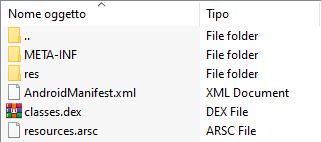
\includegraphics[width=0.6\textwidth]{imgs/capitolo2/Applicazioni/apk ins.png}
        \caption{Apk package}
        \label{fig:apkPack}
        \end{figure}
    \FloatBarrier %  evitare che i float appaiano oltre un certo punto nel tuo documento %
\subsubsection{Classes.dex}    
Questo file è composto dall'insieme delle classi che compongono la logica dell'applicativo android. Il risultato sono classi compilate dell'Android SDK per essere eseguite dalla macchina virtuale Android RunTime (ART). Trovandoci in ambiente si sviluppo java, si ha che ogni classe sarà compilata in un file .class, questo passaggio avviene anche in Android a cui però segue la conversione di tutti i file .class in un unico file .dex. Dunque questo file non conterrà il bytecode\footnote{Il bytecode è un linguaggio intermedio che si posiziona tra il linguaggio macchina e il linguaggio di programmazione. Viene adoperato per descrivere le operazioni che costituiscono un programma.} java, ma il bytecode DEX che è stato introdotto appositamente per il sistema android in quando, tra le altre, va ad ottimizzare l'uso della memoria.
\subsubsection{Res e resurces.arsc}
Nell'package apk troviamo una cartella \textit{res}, questa contiene tutte le risorse dell'applicativo come le immagini ed il layout dei file xml. Mentre \textit{resurces.arsc} è un file di risorse questa volta però compilate. 
\subsubsection{META-INF}
Questa cartella contiene le informazioni del manifest ed altri metadati\footnote{Sistema di dati il cui scopo è la descrizione di altri dati, compresi gli archivi elettronici.}. Nello specifico il file \textit{MANIFEST.MF} contiene tutte quelle informazioni utilizzate da ART in fase di run-time, come ad esempio qual è la classe principale e quali sono le politiche di sicurezza. 


%%%%%%%%%%%%%%%%%%%%%%%%%%%%%%%%%%%%%%%%%%%%%%%%%%%%%%%%%%%


%%%%%%%%%%%%%%%%%%%%%%%%%%%%%%%%%%%%%%%%%%%%%%%%%%%%%%%%%%%



%%%%%%%%%%%%%%%%%%%%%%%%%%%%%%%%%%%%%%%%%%%%%%



	\chapter{Sicurezza in ambiente Android}
\label{chap:cap3}
Android, come detto, è il leader mondiale del mercato mobile, questo ha portato all'aumento dello sviluppo di diversi tipi di applicazioni aumentando di conseguenza anche il numero degli attacchi attraverso l'utilizzo di applicazioni affette da malware. Un rapporto di Avira descrive come nella prima metà del 2020 si potessero contare quasi 2 milioni di applicazioni android affette da malware\cite{newMalwareAvira} figura \ref{fig:avira}, nell'anno precedente le rilevazioni effettuate da G DATA mostravano lo stesso trend\cite{newMalware} come si può osservare in figura \ref{fig:GSATA}. 
     \begin{figure}[h]
        \centering
        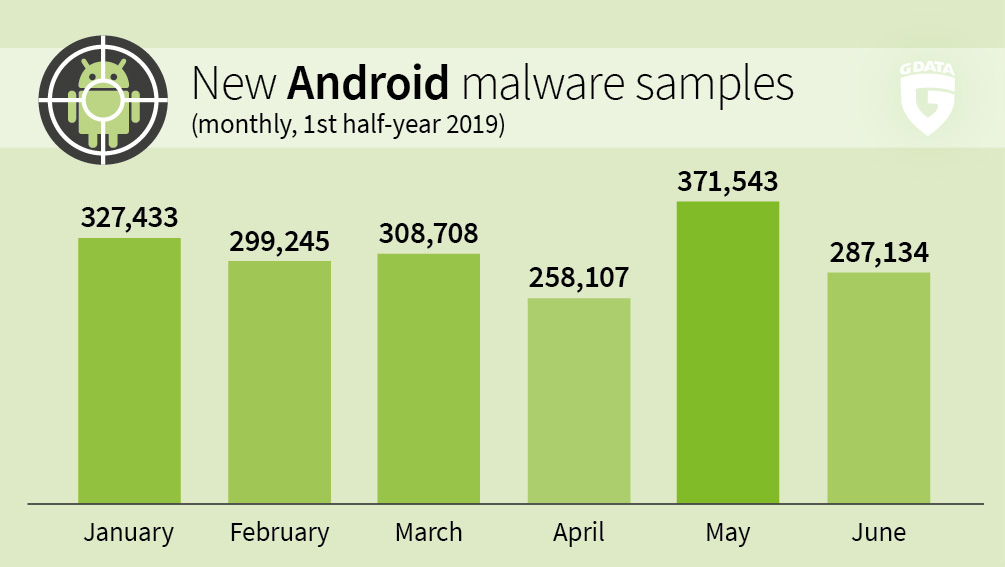
\includegraphics[width=0.6\textwidth]{imgs/capitolo3/G_DATA-Infographic-MMR-HJ1-2019-New_Android_Malware-monthly-EN-Logo.jpg}
        \caption{Malware detection 2019 - G DATA}
        \label{fig:GSATA}
\end{figure}
\FloatBarrier %  evitare che i float appaiano oltre un certo punto nel tuo documento %
\begin{figure}[h]
        \centering
        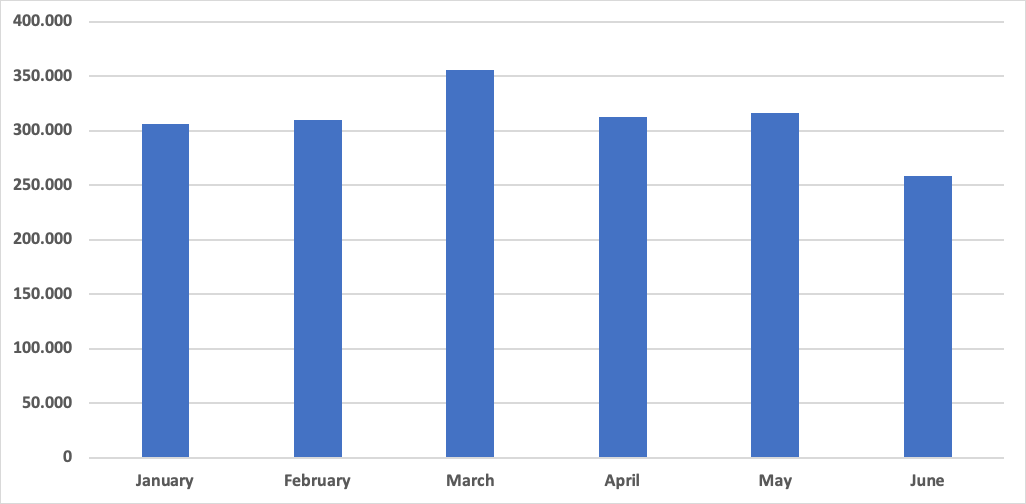
\includegraphics[width=0.6\textwidth]{imgs/capitolo3/avira.png}
        \caption{malware detection 2020 - Avira}
        \label{fig:avira}
        \end{figure}
\FloatBarrier %  evitare che i float appaiano oltre un certo punto nel tuo documento %
Il malware inoltre è stato la categoria di attacco che più è stata rilevata come minaccia in ambiente android, quasi $3/4$ delle rilevazioni riguardavano appunto un malware\cite{newMalwareAvira}.
Questo è stato reso possibile dalla frammentazione del mercato. Essendo un sistema operativo in continua evoluzione e diffusione diventa sempre più complesso riuscire a garantire la sicurezza di tutte le versioni in circolazione. Di fatti un problema per la sicurezza è legato alla versione android istallata sul proprio device. Nel 2017 si stimava ci fossero circa 1 miliardo di dispositivi android che non fossero aggiornati o non avrebbero ricevuto aggiornamenti, rendendo i dispositivi sempre più obsoleti e vulnerabili\cite{oneMilion}. 

In figura \ref{fig:os version}, nell'intervallo che va dal Gennaio 2019 al Gennaio 2021 possiamo infatti osservare come le due versioni più diffuse siano Android 9 (2017) e Android 8 (2018) 

    \begin{figure}[h]
        \centering
        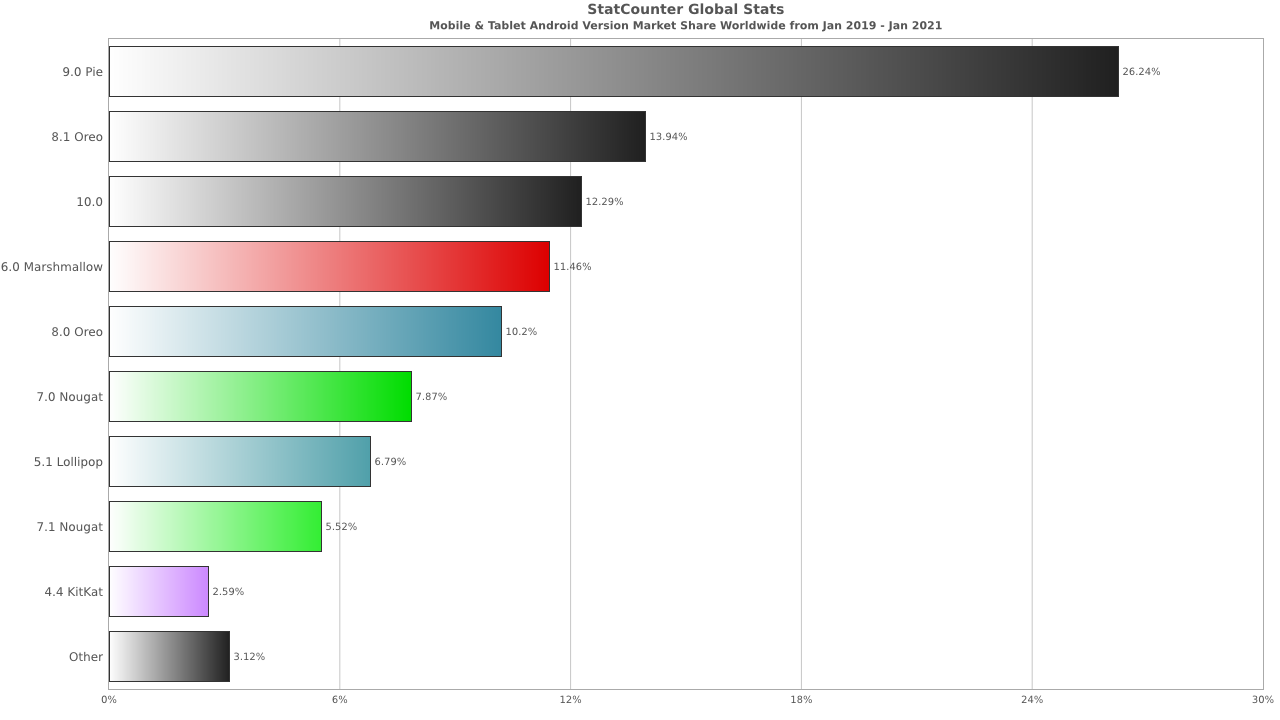
\includegraphics[width=0.6\textwidth]{imgs/capitolo3/StatCounter-android_version-ww-monthly-201901-202101-bar.png}
        \caption{Android OS Version - GlobalStats statcounter}
        \label{fig:os version}
        \end{figure}
        \FloatBarrier %  evitare che i float appaiano oltre un certo punto nel tuo documento %


Il rischio rimane quindi molto alto e da non sottovalutare. 
Nel prossimo paragrafo vedremo cosa si intende per malware. 
\section{Malware}
un Malicius software abbreviato, Malware, è un termine che va ad indicare tutti quei programmi che mettono a rischio un sistema informatico. La maggior diffusione avviene attraverso internet e più nello specifico attraverso le e-mail. In ambiente mobile però le app dannose possono nascondersi anche all'interno di applicazioni che all'apparenza sembrano non rappresentare una minaccia, questo avviene soprattutto se ci si affida per il download a store non ufficiali. I tipi di malware più diffusi sono: 
\begin{itemize}
    \item \textit{Virus}: programmi presenti in applicazini che una volta eseguite diffondono il codice malevole ad altri programmi del sistema;
    \item \textit{Trojan}: codice che solitamente è nascosto in applicazioni che riusltano utili all'utente ma che una volta istallate consentono agli attaccanti di ottenere l'accesso al dispositivo; 
    \item \textit{Ransomware}: impediscono all'utente di accedere al proprio dispositivo cifrando i suoi file, spesso sono seguiti da una richiesta di riscatto per riottenere l'accesso al dispositivo; 
    \item \textit{Worm} si diffondono nei dispositivi di una rete danneggiandoli mediante la distruzione di dati e file;
\end{itemize}

Da un'indaggine condotta da AV-Test, i trojan sono risultati il mezzo preferito dai criminali informatici per introdurre codice malevolo rappresentando il 93.93\%  di tutti gli attacchi di malware sui sistemi Android. Il ransomware si è classificato al secondo posto, con il 2,47\% \cite{trojan}.

\subsection{Colluding}
Le applicazioni colludono perché si scambiano informazioni attraverso shared\_preferences, broadcast, external\_storage, quindi ogni set ha due applicazioni che sono in comunicazione tra loro. Le app di get salvano l'informazione mentre quelle di put ricevono l'informazione e la vanno a modificare.  
\textbf{TODO: INTEGRARE}


\textbf{Francesco: parliamo di colluding, dicendo gli attacchi che dopo andremo a testare, il fattoc he la tua metolodgia applica il multiple instance learning per rilevare applicazioni collusive deve essere chiaro sin dall' inizio della tesi}
	\chapter{La metodologia}
In questo capitolo esporremo la metodologia utilizzata per la classificazione dei file audio, nello specifico partiremo dai software e i tipi di dati utilizzati per poi muverci verso l'estrazione delle feature la generazione dei dataset e la classificazione attraverso una particolare tecnica di machine learning chiamata multiple instance learning (MIL). 
\begin{figure}[h]
\centering
    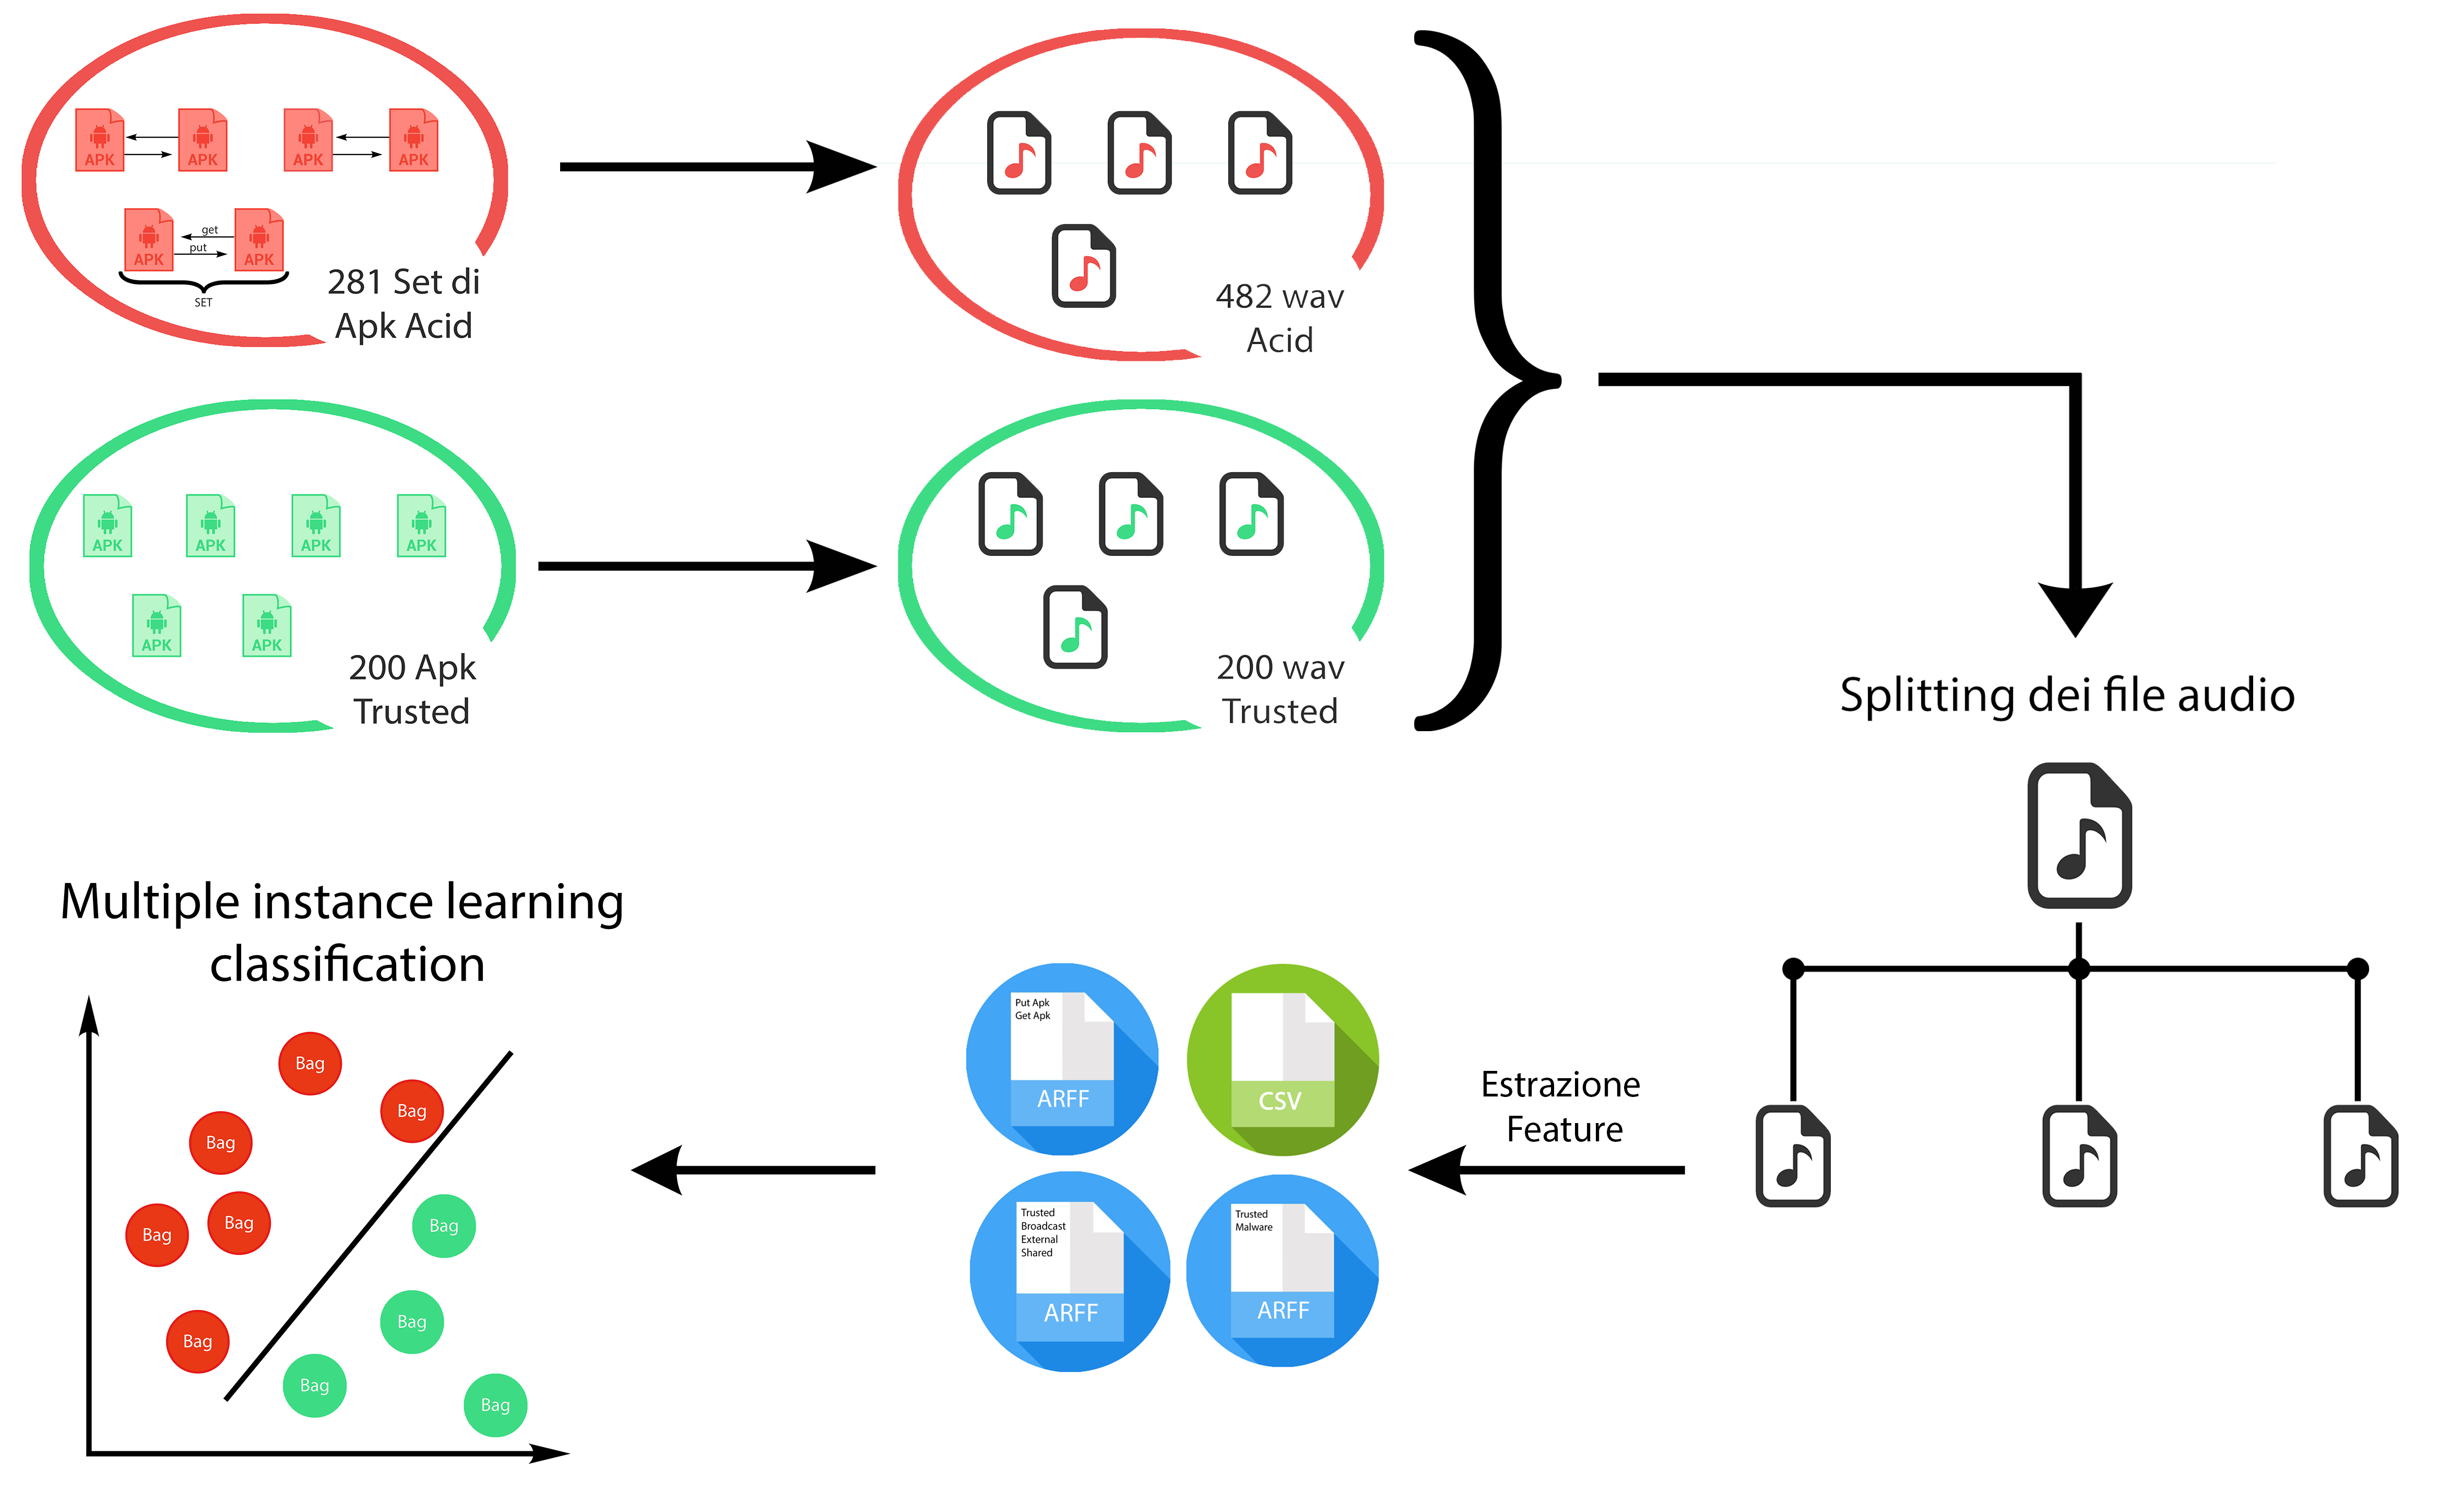
\includegraphics[width=0.9\linewidth]{imgs/capitolo4/all.png} 
    \caption{project}
    \label{fig:all}
\end{figure}
\FloatBarrier
\section{I software e i dataset}
In questo paragrafo esporremo dapprima tutti i software utilizzati nell'analisi e una breve panoramica sulle caratteristiche principali dei dataset utilizzati.  
\subsection{WEKA}
Acronimo di "Waikato Environment for Knowledge Analysis", è un software open source per il machine learning. Partendo da un dataset\footnote{Collezione di dati organizzati, la grandezza è data dal numero di righe.} è possibile applicarvi dei metodi di apprendimento automatico e di analizzarne il risultato è inolttre possibile attraverso l'utilizzo di questi metodi avere una previsione su nuovi set di dati. Per poter utilizzare gli algoritmi di classificazione del multiple instance learning bisogna importare i relativi package, attravero il tool "Package Manager" già presente di default nella schermata iniziale di weka. Figura \ref{fig:mil pckg}.
\begin{figure}[h]
\centering
    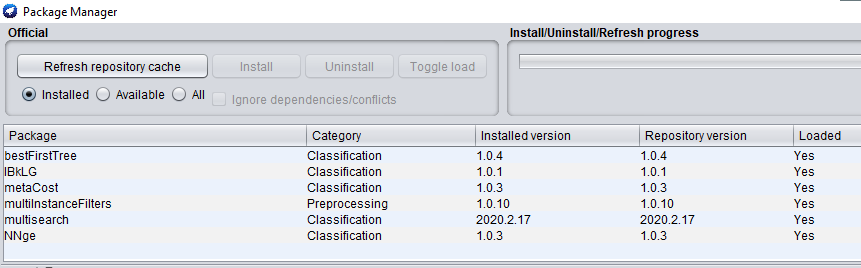
\includegraphics[width=0.9\linewidth]{imgs/capitolo4/packmil.png} 
    \caption{Imput Mil package in weka}
    \label{fig:mil pckg}
\end{figure}
\FloatBarrier
Una particolarità di questo software è l'utilizzo di dataset .arff 


\subsection{dataset.csv e dataset.arff}
I dataset utilizzati nel progetto sono dataset con estensione \textbf{.csv - Comma Separated Values}, questo è un formato di file di testo in cui ogni riga rappresenta un record della tabella. Ogni colonna invece rappresenta dei valori associati ad ogni record. le colonne sono separate da virgole, da qui il nome. In figura \ref{Fig:Datacsv} è possibile osservarne un esempio. 
\vspace{1em}
\newline
Il secondo tipo di dataset che abbiamo utilizzato sono file dati con estensione \textbf{.arff - Attribute Relationship File Format} come suggerisce il nome, questo formato di file organizza i dati seguendo una logica relazionale.
La formattazione del dataset utilizzato riguarda è stata svolta in ottica di una classificazione attraverso algoritmi di multiple instance learning, dunque si è reso necessario dover organizzare i dati in bag. L'inizializzazione del file, per una classificazione MIL\footnote{Mil - Multiple instance learning} può essere suddiviso in cinque componenti\cite{wekaDoc}:  
\begin{enumerate}
        \item Nella prima va sempre definita la relazione che lega i dati attraverso l'attributo \textbf{@relation} ed un nome che descriva quello che vogliamo predire.  
        
        \item Successivamente andranno inseriti gli identificativi delle bag, ovvero utilizzando \textbf{@attribute bag\_id \{...\}} si vanno ad inserire nelle parentesi graffe la lista di tutti gli identificative delle istanze della bag. Ogni identificativo va separato dall'altro tramite tramite l'utilizzo di una virgola. 
        
        \item Dopo si definiranno gli attributi della bag, per farlo si utilizzano\textbf{@attribute bag relational} per definire l'inizio della bag ed \textbf{@end bag}per definire la fine della bag. All'interno, tra i due attributi, vanno specificati gli attributi che compongono le istanze di una bag, ovvero le caratteristiche dei dati. Per farlo si utilizza ancora una volta l'identificativo \textbf{@attribute nome\_caratteriustica tipo\_caratteristica}. Il tipo di caratteristica può essere \textit{numeric} se il valore del dato è un numero intero, altrimeti \textbf{real} se il tipo di attributo è un numero reale altriment se il tipo di dato da rappresentare è una stringa scriveremo i valori ammissibili presenti tra parentesi graffe es. {\{yes, no\}} nel caso di un attributo booleano.
        
        \item A questo punto dobbiamo definire la classe che rappresenta una istanza. Per farlo inseriremo i valori tra parentesi graffe definendo l'attributo class come, \textbf{@attribute class {calss1, class2}}
        
        \item Infine attraverso a capo della key \textbf{@data} inseiremo il dataset correttamente formattato nel seguente modo: iesima bag\_id + ',' poi dovremmo definire tutte le istanze della bag. Una bag si definisca allinterno delle virgolette "...". All'intero delle virgolette inseiremo tutte le istanze ognuna della quali sara separata dal carattere speciale '$\backslash$n'. A loro volta ogni istanza è rappresentata dai diversi attributi, tanti quanti ne abbiamo definiti in precedenza, ogni attributo d'istanza è separato dall'altro tramite ','. Infine dopo la chiusura delle virgolette inseriamo la virgola e va definita la classe della bag. Ogni riga ha quindi la seguente formattazione:
        \\\footnotesize {
        bag\_id , " attr1Ist1, attr2Ist1, attr3Ist1 $\backslash$n attr1Ist2, attr2Ist2, attr3Ist2 $\backslash$n attr1Ist3, attr2Ist3, attr3Ist3 " , classe  }
    \end{enumerate}
\begin{figure}[h]
   \begin{minipage}{0.48\textwidth}
     \centering
     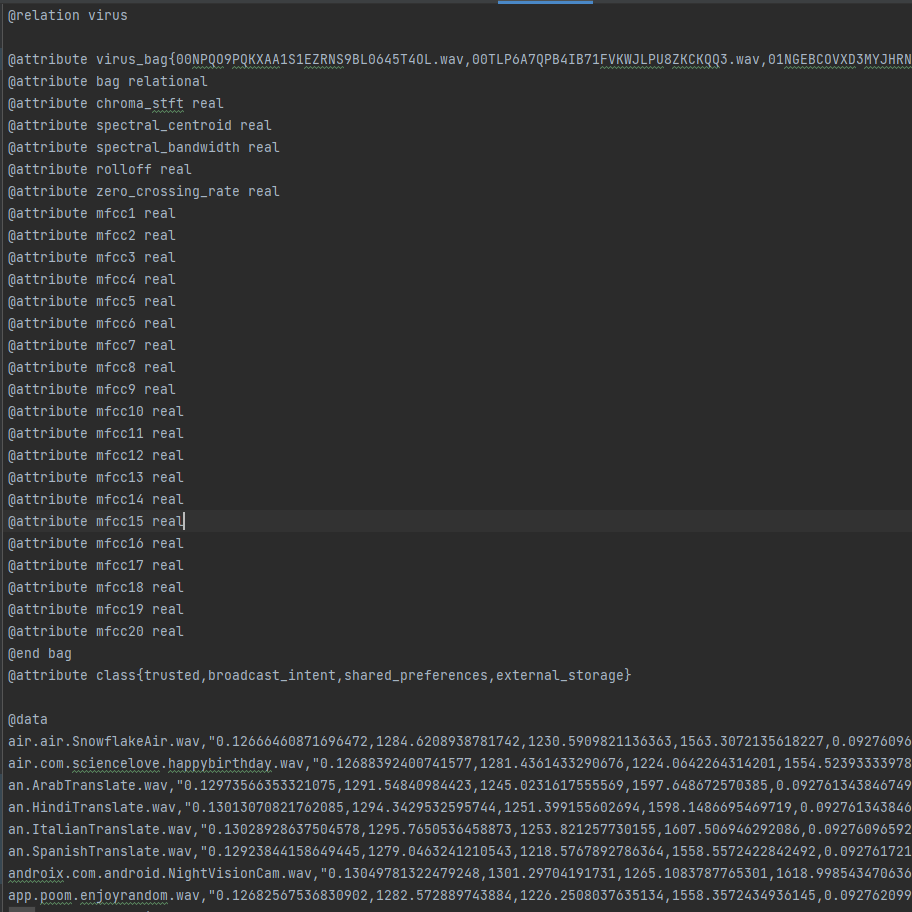
\includegraphics[width=0.85\linewidth]{imgs/capitolo4/ARFF.png}
     \caption{ARFF dataset for MIL}
     \label{Fig:Dataarff}
   \end{minipage}\hfill
   \begin{minipage}{0.48\textwidth}
     \centering
     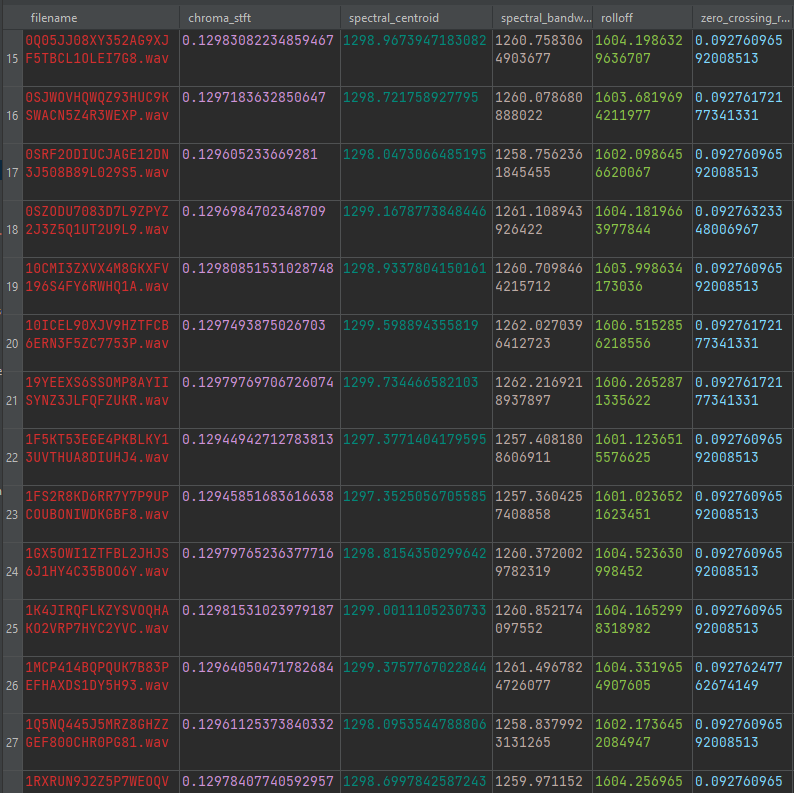
\includegraphics[width=0.85\linewidth]{imgs/capitolo4/csv.png}
     \caption{CSV file}
     \label{Fig:Datacsv}
   \end{minipage}
\end{figure}
\FloatBarrier 
\subsection{dataset di applicativi andorid}
Siamo partiti da due dataset di applicazioni apk. La prima conteneva un set di 200 applicazioni andorid non affette da malware che abbiamo definito il dataset come "trusted", il secondo dataset invece conteneva 241 applicazioni affette da malware abbiamo definito questo dataset come "Acid". TODO:...
\section{Elaborazione dei file audio}
In questo paragrafo descriveremo l'elaborazione dei file audio, coem sono stati generati e suddivisi.

	% Inserite qui gli altri capitoli:
	%\input{miocapitolo1}
	%\input{miocapitolo2}
	%%%%%%%%%%%%%%%%%%%%%%%%%%%%%%%%%%%%%%%%%%%%%%%%%%%%%%%%%%%

\chapter{Conclusioni}
\label{chap:Conclusioni}

\begin{flushright}
\textit{Ing.Francesco Mercaldo, Dott.ssa Rosangela Casolare , Andrea D'Aguanno} 
\end{flushright}
	

	% === Bibliografia ====================================
	\newpage
	\bibliographystyle{IEEEtran}
	\bibliography{bibliografia-tesi.bib}

\end{document}

%%%%%%%%%%%%%%%%%%%%%%%%%%%%%%%%%%%%%%%%%%%%%%%%%%%%%%%%%%%
